% libraries:
% Clipping to a circle, a rectangle in a scope, and an intersection of clips.
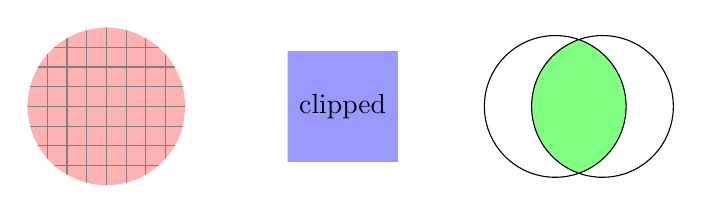
\begin{tikzpicture}
  \begin{scope}
    \clip (1,1) circle (1);
    \fill[red!30] (0,0) rectangle (2,2);
    \draw[step=0.25, gray] (0,0) grid (2,2);
  \end{scope}
  \begin{scope}[xshift=3cm]
    \clip (0.3,0.3) rectangle (1.7,1.7);
    \fill[blue!40] (1,1) circle (1);
    \node at (1,1) {clipped};
  \end{scope}
  \begin{scope}[xshift=6cm]
    \clip (0.7,1) circle (0.9);
    \clip (1.3,1) circle (0.9);
    \fill[green!50] (0,0) rectangle (2,2);
  \end{scope}
  \draw (6.7,1) circle (0.9) (7.3,1) circle (0.9);
\end{tikzpicture}
